
%(BEGIN_QUESTION)
% Copyright 2012, Tony R. Kuphaldt, released under the Creative Commons Attribution License (v 1.0)
% This means you may do almost anything with this work of mine, so long as you give me proper credit

Examine this process, where the temperature of water sitting at the bottom of a ``water seal drum'' vessel is regulated by passing hot steam through a heating tube immersed in the water:

$$\includegraphics[width=15.5cm]{i0002rx01.eps}$$

Suppose that one day the 30 PSI steam supply boiler shuts down, ceasing the flow of steam to the TV-26.  With no supply of steam to heat the seal drum, the water begins to cool down.  What will controller TC-26 do in response to this event, assuming it is a proportional+integral (P+I) controller?  

Now suppose that the steam ``outage'' lasts for a very long time.  How will the controller's proportional and integral modes respond if left in the automatic mode the entire time?  Is there a way to avoid this problem?
 
\vskip 20pt \vbox{\hrule \hbox{\strut \vrule{} {\bf Suggestions for Socratic discussion} \vrule} \hrule}

\begin{itemize}
\item{} Examining the diagram, what do you suppose the function of the water seal drum is, in the larger context of the flare process?
\item{} Which is the worst-case scenario: the water in the seal drum becoming too cold or becoming too hot?  How can we tell based on details found in this diagram?
\item{} Suppose operations personnel approached you to install instrumentation to measure the total quantity of substance released to the flare each month, for emissions monitoring purposes.  For those who have studied flowmeters, identify at least one practical solution to this problem, including the specific types of technologies used to sense the vapors going to the flare.
\end{itemize}

\underbar{file i01608}
%(END_QUESTION)





%(BEGIN_ANSWER)

The controller will decrease its output signal as it tries to open the air-to-close valve.  Both the proportional and integral terms of the controller will work to open the steam valve as the reactor temperature decreases.  If there is no steam supply for an extended period of time, the controller's integral action will {\it wind} to a condition of saturation (3 PSI or less output signal pressure).

%(END_ANSWER)





%(BEGIN_NOTES)

Of course, the seal drum water will not heat back up until steam supply is re-established, no matter what position the controller sets the steam control valve to.

Integral ``windup'' may be re-set by placing the controller in manual and then switching back to automatic.  Internal ``windup limits'' may be set to help prevent this from happening in the future.

\vskip 10pt

One solution to the Socratic Question of how to measure total substance quantity flared is to place an ultrasonic flowmeter in the flare line, then totalize (integrate) that flow measurement.  Another solution would be to measure the radiant heat output by the flame, integrating that (to calculate total BTU burned).











\filbreak \vskip 20pt \vbox{\hrule \hbox{\strut \vrule{} {\bf Virtual Troubleshooting} \vrule} \hrule}

\noindent
{\bf Predicting the effect of a given fault:} present each of the following faults to the students, one at a time, having them comment on all the effects each fault would produce.

\begin{itemize}
\item{} 
\item{} 
\item{} 
\end{itemize}


\vskip 10pt


\noindent
{\bf Identifying possible/impossible faults:} present symptoms to the students and then have them determine whether or not a series of suggested faults could account for all the symptoms, explaining {\it why} or {\it why not} for each proposed fault:

\begin{itemize}
\item{} Symptom: {\it }
\item{} 
\item{} 
\item{} 
\end{itemize}


\vskip 10pt


\noindent
{\bf Determining the utility of given diagnostic tests:} present symptoms to the students and then propose the following diagnostic tests one by one.  Students rate the value of each test, determining whether or not it would give useful information (i.e. tell us something we don't already know).  Students determine what different results for each test would indicate about the fault, if anything:

\begin{itemize}
\item{} Symptom: {\it }
\item{}  -- {\bf Yes/No}
\item{}  -- {\bf Yes/No}
\end{itemize}


\vskip 10pt


\noindent
{\bf Diagnosing a fault based on given symptoms:} imagine the nozzle plugs in LC-21, causing the level control valve to open wide and flood the water seal drum with water (don't reveal the fault to students!).  Present the operator's observation(s) to the students, have them consider possible faults and diagnostic strategies, and then tell them the results of tests they propose based on the following symptoms, until they have properly identified the nature and location of the fault:

\begin{itemize}
\item{} {\it Operators receive a high level alarm LAH-22}
\item{} LT-21 receiver gauge shows 16 PSI
\item{} LV-21 is wide open
\item{} TC-26 is below setpoint (PV = 50 deg F ; SP = 100 deg F)
\item{} PG-36 and PG-37 both are showing oscillating pressure readings (occasional surges)
\item{} {\it First step(s) to take once the problem has been identified?}
\end{itemize}


%INDEX% Control, integral: windup
%INDEX% Process: steam-heated reactor vessel (generic)

%(END_NOTES)


